\documentclass[a4paper]{article}

\usepackage[english]{babel}
\usepackage{amsmath}
\usepackage{amssymb}
\usepackage{dsfont}
\usepackage{tikz}
\usetikzlibrary{arrows,automata}
\title{Calculus and Probability Theory\\ Assignment 3}
\author{Christoph Schmidl\\
s4226887\\
Informatica\\
c.schmidl@student.ru.nl\\
Exercise Teacher: Gergely Alp\'{a}r}

\date{\today}

\begin{document}
\maketitle

\begin{enumerate}

\item (\textbf{15 points}) As we learnt in the lecture (slide 33), the function arccos is the inverse function of cos.

\begin{enumerate}
	\item[(a)] What it the domain of the function arccos(x)? Why?\\
	\textbf{Solution:}\\
	
As we already know from the cosine function, the domain of the cosine function is $\mathbb{R}$ and its range is $[-1,1]$	
	
\begin{figure}[ht]
	\centering
  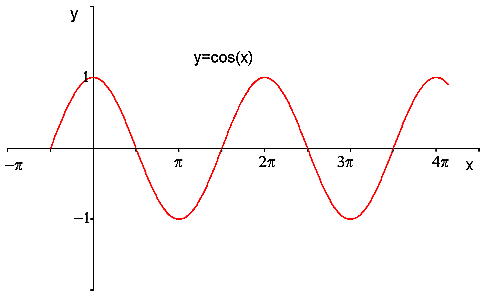
\includegraphics[width=0.6\textwidth]{cosine.png}
\end{figure}	
	
An Inverse function is a function that "reverses" another function: if the function $f$ applied to an input $x$ gives a result of $y$, then applying its inverse function $g$ to $y$ gives the reult $x$ and vice versa.\\

Let $f$ be a function whose domain is the set $X$ and whose range is the set $Y$. Then $f$ is invertible if there exists a function $g$ with domain $Y$ and $range$ $X$, with property 

\begin{equation}
	f(x) = y \leftrightarrow g(y) = x \notag
\end{equation}	
	
Because we already know, that arccos is the inverse function of cosine, its domain has to be the range of cosine, which is $[-1,1]$.	
	
	\item[(b)] Compute the following values and explain how you got the result:\\
	
	\begin{itemize}
		\item $arccos(1) = ?$\\
		\textbf{Solution:}\\
\begin{align*}
	\arccos x = \theta \\
	\cos \theta = x
\end{align*}

Question: What angle $\theta$ can i take the cosine of to get $x$?\\ 

\begin{align*}
	\arccos(1) = \theta\\
	\cos \theta = 1
\end{align*}

\begin{figure}[ht]
	\centering
  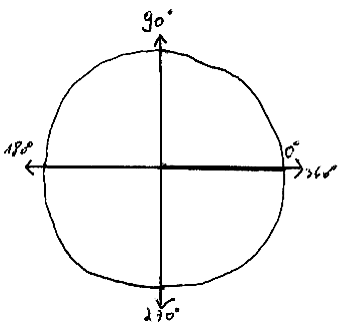
\includegraphics[width=0.4\textwidth]{c1.png}
\end{figure}


From the picture of the cosine function in 1a) it is easy to see that the $arccos(1)$ is $0$. We can also take a look at the unit circle and read it that way.\\

				\item $arccos(0) = ?$\\
				\textbf{Solution:}\\
		
\begin{align*}
	\arccos x = \theta \\
	\cos \theta = x
\end{align*}

Question: What angle $\theta$ can i take the cosine of to get $x$?\\ 

\begin{align*}
	\arccos(0) = \theta\\
	\cos \theta = 0
\end{align*}

\begin{figure}[ht]
	\centering
  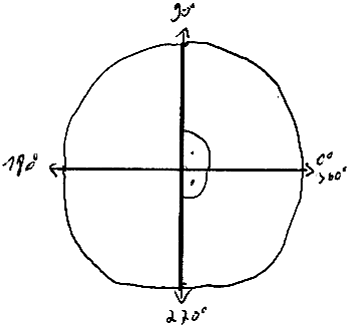
\includegraphics[width=0.4\textwidth]{c2.png}
\end{figure}

Again, we can just read the answer from the cosine function in 1a) and ask: where does the cosine function hit the x-axis? And the answer is $\frac{\pi}{2}$.\\

Another explanation can be taken from the unit circle. If we let the cosine be 0, then there is an angle of $90$. Therefore:\\

$90 \cdot \frac{\pi}{180} = \frac{\pi}{2}$\\


		\item $arccos(\frac{\sqrt{3}}{2}) = ?$\\
		\textbf{Solution:}\\
\begin{align*}
	\arccos x = \theta \\
	\cos \theta = x
\end{align*}

Question: What angle $\theta$ can i take the cosine of to get $x$?\\ 

\begin{align*}
	\arccos(\frac{\sqrt{3}}{2}) = \theta\\
	\cos \theta = \frac{\sqrt{3}}{2}
\end{align*}		
		
\begin{figure}[ht]
	\centering
  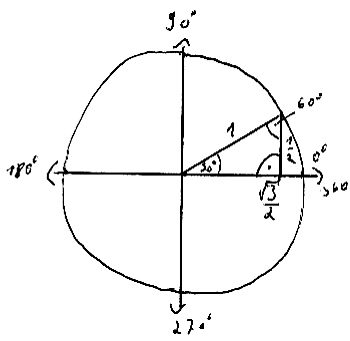
\includegraphics[width=0.4\textwidth]{c3.png}
\end{figure}		
	\end{itemize}
	
In this scenario, we have to work with the unit circle. We know, we have to draw the length of the arccos to be $\frac{\sqrt{3}}{2}$ as we see in the picture.\\ After that, we can use pythagoras' theorem to compute the opposite/adjacent, which givues us $\frac{1}{2}$. We already know that the hypothenuse is 1, because it's a unit circle.\\

After that, we get an angle of 30 and therefore:\\

$30 \cdot \frac{\pi}{180} = \frac{\pi}{6}$\\
	
	\item[(c)] Find the derivative of f:\\
	
	\begin{equation}
		f(x) = arccos(\frac{2x}{1 - x})\notag
	\end{equation}
	
	\textbf{Solution:}\\
	
	\begin{equation}
		(\arccos x)' = \frac{-1}{ \sqrt{1 - x^2}} \notag
	\end{equation}	
	
Using the chain rule $ \frac{d}{dx}(cos^{-1}(\frac{2x}{1-x})) = \frac{d \cos^{-1}(u)}{du} \frac{du}{dx}$, where $u = \frac{2x}{1 - x}$ and $\frac{d}{du} (\cos^{-1}(u)) = -\frac{1}{\sqrt{1 - u^2}}$\\

$= - \frac{2 \frac{d}{dx}(\frac{2x}{1-x})}{\sqrt{1 - \frac{4x^2}{(1-x)^2}}}$	\\

Use the quotient rule, $\frac{d}{dx}(\frac{u}{v}) = \frac{v \frac{du}{dx} - u \frac{dv}{dx}}{v^2}$ where $u = x$ and $v = 1 - x$\\

$= - \frac{2((1-x)(\frac{d}{dx}(x)) - \frac{d}{dx}(1) - \frac{d}{dx}(x))}{(1 - x)^2 \sqrt{1 - \frac{4x^2}{(1-x)^2}}}$	

$= -\frac{2(x + 1 (1-x))}{(1-x)^2   \sqrt{1 - \frac{4x^2}{(1-x)^2}}}$
	
$= - \frac{2}{(1-x)^2 \sqrt{1 - \frac{4x^2}{(1-x)^2}}}$	
	
	
\end{enumerate}
\newpage
\item (\textbf{15 points}) Given the functions $f(x) = log_2(4x)$ and $g(x) = sin(2x)$.

	\begin{enumerate}
		\item[(a)] What is $f'''(x)$?\\
\textbf{Solution:}\\


\begin{align*}
\frac{d}{dx}(\log_2(4x)) = \log_2(4x)' &= \frac{\frac{d}{dx}(ln(4x))}{ln(2)}\\
&= \frac{\frac{\frac{d}{dx}(4x)}{4x}}{\ln(2)}\\
&= \frac{4 \frac{d}{dx}(x)}{4x \ln(2)}\\ 
&= \frac{\frac{d}{dx}(x)}{x \ln(2)}\\
&= \frac{1}{x \ln(2)}
\end{align*}

\begin{align*}
	\frac{d}{dx}(\frac{1}{x \ln(2)}) = \log_2(4x)'' &= \frac{\frac{d}{dx}(\frac{1}{x})}{\ln(2)}\\
	&= \frac{\frac{-1}{x^2}}{\ln(2)}\\
	&= -\frac{1}{x^2 \ln(2)}
\end{align*}
		
		
\begin{align*}
	\frac{d}{dx}(-\frac{1}{x^2 \ln(2)}) = \log_2(4x)''' &= -\frac{\frac{d}{dx}(\frac{1}{x})}{\ln(2)}\\
	&= -\frac{\frac{-1}{x^2}}{\ln(2)}\\
	&= \frac{1}{x^2 \ln(2)}
\end{align*}		
		
		
		\item[(b)] What is $g^{(2014)}(x)$\\
		\textbf{Solution:}\\
		
$\sin(2x)' = \frac{d}{dx}(\sin(2x)) = \cos(2x)(\frac{d}{dx}(2x)) = 2 \cos(2x)$\\

$\sin(2x)'' = \frac{d}{dx}(2 \cos(2x)) = -4 \sin(2x)$\\

$\sin(2x)''' = \frac{d}{dx}(-4 \sin(2x)) = -8 \cos(2x)$\\	
		
$\sin(2x)'''' = \frac{d}{dx}(-8 \cos(2x)) = 16 \sin(2x)$\\

$g^{2014}(x) = 2^{2014} \cdot (-\sin(2x))$\\
		
	\end{enumerate}
	
	
\item (\textbf{25 points}) Investigate function $f = (x-1)^2(x+2)$ by following the steps below. (Do not start with drawing a graph by means of a device or some web resource. Of course you may check your result when you are done.) 
	
	\begin{enumerate}
			\item[(a)] Determine the domain of function $f$.\\
			
$D(f(x)) = \{ x \in \mathbb{R}\}$\\				
			
			
			
			\item[(b)] What are the roots of $f$? Where does the graph of $f$ intersect the $y$ axis?\\
			
$f = (x-1)^2(x+2) = x^3 - 3x + 2$\\
$x^3 - 3x + 2 = 0$\\			

First root by guessing: $1^3 - 3 + 2 = 1 - 3 + 2 = 0$\\
$x = 1$\\

Polynomdivision: $(x^3 - 3x +2): (x - 1) = x^2 + x - 2$\\

ABC-Formula: $ax^2 + bx + c = 0 \rightarrow x = \frac{-b + \sqrt{b^2 - 4ac}}{2a} $ or $\frac{-b - \sqrt{b^2 - 4ac}}{2a}$\\

$x^2 + x - 2 = 0 \rightarrow x = \frac{-1 - \sqrt{1^2 + 8}}{2} = \frac{-1 - 3}{2} = -2$\\

Roots:

\begin{align*}
	x &= -2\\
	x&= 1
\end{align*}			
		
Intersection with y-axsis: $f(0)	= 0^3 - 3 \cdot 0 + 2 = 2$\\	
		
			
			
			\item[(c)] Determine the limits at the edges of the domain. In this case, there are only two edges:
			
			\begin{equation}
			\lim_{x \to -\infty}f(x) \qquad and \qquad \lim_{x \to + \infty}f(x) \notag
			\end{equation}
			
			\item[(d)] Find $f'$ and $f''$.\\

$f = (x - 1)^2{x + 2} = x^3 - 3x + 2$\\
$f' = \frac{d}{dx}(x^3 - 3x + 2) = 3x^2 - 3 = x(x^2 - 1)$\\		
		
$f'' = \frac{d}{dx}(3x^2 - 3) = 6x$\\			
			
			
			\item[(e)] Find the zeros of $f'$ and $f''$.\\
			
			
\begin{align*}
 f'' = x(x^2-1) \rightarrow x(x^2-1) = 0\\
\end{align*}				
			
	
Roots: $x = -1, x = 0, x = 1$\\	
			
			
\begin{align*}
 f'' = 6x \rightarrow 6x = 0\\
\end{align*}			

Roots: $x = 0$
			
			
			
			\item[(f)] What are the critical points (determine their $x$ and $y$ coordinates)?\\
			
			\item[(g)] Find the local minimums and maximums.\\
			
			\item[(h)] Which parts of the function are convex and concave? Does the function $f$ have points of inflection? (Hint: Use the sign of the second derivative for answering both questions.)\\
			
			\item[(i)] Draw the graph of function $f$. (If you collect all intervals and special points in a table, it helps a lot in drawing the graph. Moreover, you get some extra points!)\\		
			
			
			
	\end{enumerate}		
	
\item (\textbf{25 points}) We will sketch the function 

\begin{equation}
	f(x) = \frac{x^2}{x - 2} \notag
\end{equation}
	
following similar steps as the ones in the previous problem. Additionaly, we prove that the line $y = x + 2$ is an asymptote on both sides. (Again, do not start with drawing a graph by means of a device or some web resource. Of course you may check your result when you are done.)


	\begin{enumerate}
		\item[(a)] Determine the domain of function $f$.\\
		
$D(f(x)) = \{ x \in \mathbb{R} | x \neq 2\}$\\		
		
		
		\item[(b)] What are the roots of $f$? Where does the graph of $f$ intersect the $y$ axis?\\
		
		
Roots:\\

\begin{align*}
	\frac{x^2}{x - 2} &= 0\\
	\frac{x^2}{x - 2}  \cdot (x - 2) &= 0\\
	x^2 &= 0\\
	x &= 0
\end{align*}	
		
The only root is $x = 0$\\
		
		
Intersection with y-axsis: $f(0) = \frac{0^2}{0 - 2} = 0$\\

		
		\item[(c)] Determine the limits at the edges of the domain.\\
		
		\item[(d)] Find $f'$ and $f''$.\\
		

\begin{align*}
	f' &= \frac{d}{dx}(\frac{x^2}{x - 2})\\
	&= \frac{-x^2(\frac{d}{dx}(-2+x)) + (-2 + x)(\frac{d}{dx}(x^2)}{(-2+x)^2}\\
	&= \frac{-(x^2 (\frac{d}{dx}(x))) + (-2 + x)(\frac{d}{dx}(x^2))}{(-2 + x)^2}\\
	&= \frac{(-2 + x)(\frac{d}{dx}(x^2)) - x^2}{(-2 + x)^2}\\
	&= \frac{-x^2 + (-2 + x) 2x}{(-2 + x)^2}\\
	&= \frac{(x-4)x}{(x - 2)^2}
\end{align*}		
		
		
\begin{align*}
	f'' &= \frac{d}{dx}(\frac{(x - 4)x}{(x - 2)^2})\\
	&= \frac{x(\frac{d}{dx}(-4 + x))}{(-2 + x)^2} + (-4 + x) (\frac{d}{dx}(\frac{x}{(-2 + x)^2}))\\
	&= \frac{x}{(-2 + x)^2} + (-4 + x)(\frac{d}{dx}(\frac{x}{(-2 + x)^2}))\\
	&=  \frac{x}{(-2 + x)^2} + (-4 + x) (\frac{\frac{d}{dx}(x)}{(-2 + x)^2} + \frac{-2 \frac{d}{dx}(-2 + x)}{(x - 2)^3}x)\\
	&= \frac{x}{(-2 + x)^2} + (-4 + x) (\frac{1}{(-2 + x)^2} - \frac{2x}{(-2 + x)^3})\\
	&= \frac{8}{(x - 2)^3}
\end{align*}
		
		
		\item[(e)] Find the zero of $f'$ and $f''$.\\
		
		
\begin{align*}
 f' = \frac{(x-4)x}{(x-2)^2} \rightarrow \frac{(x-4)x}{(x-2)^2} = 0\\
\end{align*}		
		
Roots for $f'$: 		
		
		\begin{align*}
	x &= 0\\
	x &= 4
\end{align*}

\begin{align*}
 f'' = \frac{8}{(x - 2)^3} \rightarrow \frac{8}{(x - 2)^3} = 0\\
\end{align*}

Roots for $f''$: No roots exist.

		
		\item[(f)] What are the critical points (determine their $x$ and $y$ coordinates)?\\
		
		\item[(g)] Find the local minimums and maximums.\\
		
		\item[(h)] Which parts of the function are convex and concave? Does function $f$ have points of inflection? (Hint: Use the sign of the second derivative for answering both questions.)
		
		\item[(i)] Show that the line $y = x + 2$ is a slant asymptote of $f$. (Hint: Use the definition on slide 41 of the lecture and the following two limits.)
		
		\begin{equation}
		\lim_{x \to - \infty}(f(x) - (x+2)) = ? \qquad and \qquad \lim_{x \to + \infty} (f(x) - (x+2)) = ?\notag
		\end{equation}				
		
		\item[(j)] Draw the graph of function $f$.\\
				
		
	\end{enumerate}		
	
	
\item (\textbf{12 points}) Given function f, find the partial derivatives. If it is necessary, simplify the result.\\

	\begin{enumerate}
		\item[(a)] $f(x,y) = \sin(3x + 3xy)$; $\frac{\partial f(x,y)}{\partial x}= ?$ and $\frac{\partial f(x,y)}{\partial y} = ?$\\
		
		\item[(b)] $f(x,y) = \ln(\frac{y}{x})$; $\frac{\partial f(x,y)}{\partial x}= ?$ and $\frac{\partial f(x,y)}{\partial y} = ?$\\
	\end{enumerate}
	
	
\item (\textbf{8 points}) If $f(x,y) = \frac{xy}{x - y}$, show that 

\begin{equation}
	x^2 \frac{\partial^2 f(x,y)}{\partial x^2} + 2xy \frac{\partial^2 f(x,y)}{ \partial x \partial y} + y^2 \frac{\partial^2 f(x,y)}{\partial y^2}\notag
\end{equation}	
(Hint: First compute all the second partial derivatives of $f$, then substitute the results in the expression on the left-hand side.)
	
	
	
\end{enumerate}

\end{document}
